\chapter{Manusia dan Alam}\label{ch:g5:people-and-nature}

Dari puncak bukit, pandanglah ke bawah ke arah lembahnya: ladang dalam
petak-petak rapi, hutan yang dikelola, tepian sungai yang diluruskan,
jalan, atap. Hampir tidak ada yang terlihat tumbuh sendiri seperti itu.
Manusia adalah satu-satunya \omterm{def:g5:biodiversity:species}{spesies} yang membentuk ulang seluruh
bentang alam menurut kebutuhannya --- dan bab ini memandang kekuatan
itu dengan jujur: apa yang diberikannya kepada kita, berapa harganya,
dan bagaimana ia dapat dipakai dengan baik.

\section{Bentang alam buatan manusia}

\begin{proposition}[Kebanyakan bentang alam dikelola]\label{prop:g5:people-and-nature:managed}
Nyaris setiap bentang alam di sekitar kita dibentuk manusia:
\begin{itemize}
  \item \emph{ladang}\index{ladang} adalah tanah kelolaan tempat satu
        \omterm{def:g1:plants-around-us:plant}{tumbuhan} pilihan --- gandum, jagung, kentang --- ditanam
        sebagai ganti campuran yang liar;
  \item kebanyakan \emph{hutan}\index{hutan kelolaan} ditanam,
        dijarangkan dan dipanen seperti tanaman yang lambat;
  \item \emph{padang rumput} ada karena ia dipangkas atau digembalai
        --- kalau ditinggalkan, ia tumbuh kembali menjadi semak
        belukar lalu menjadi hutan;
  \item kota, jalan dan bendungan menggambar ulang tanahnya sendiri.
\end{itemize}
Sudut yang ``tak tersentuh'' adalah perkecualian, dan kebanyakan
dilindungi dengan sengaja.
\end{proposition}
\admitted

\begin{example}[Membaca lembahnya]\label{ex:g5:people-and-nature:valley}
Pemandangan dari puncak bukit itu, satu demi satu: ladang gandumnya
memberi makan toko rotinya; deretan pohon cemaranya adalah panen kayu
yang lebih tua daripada rimbawannya; padang rumput berbunganya
dipangkas setiap bulan Juli --- lewatkan dua musim panas dan semak
berduri mengambilnya; sungainya diluruskan sejak lama untuk melindungi
ladangnya dari banjir. Lembah itu adalah sebuah bengkel --- bengkel
yang sudah berjalan berabad-abad.
\end{example}

\begin{omfigure}
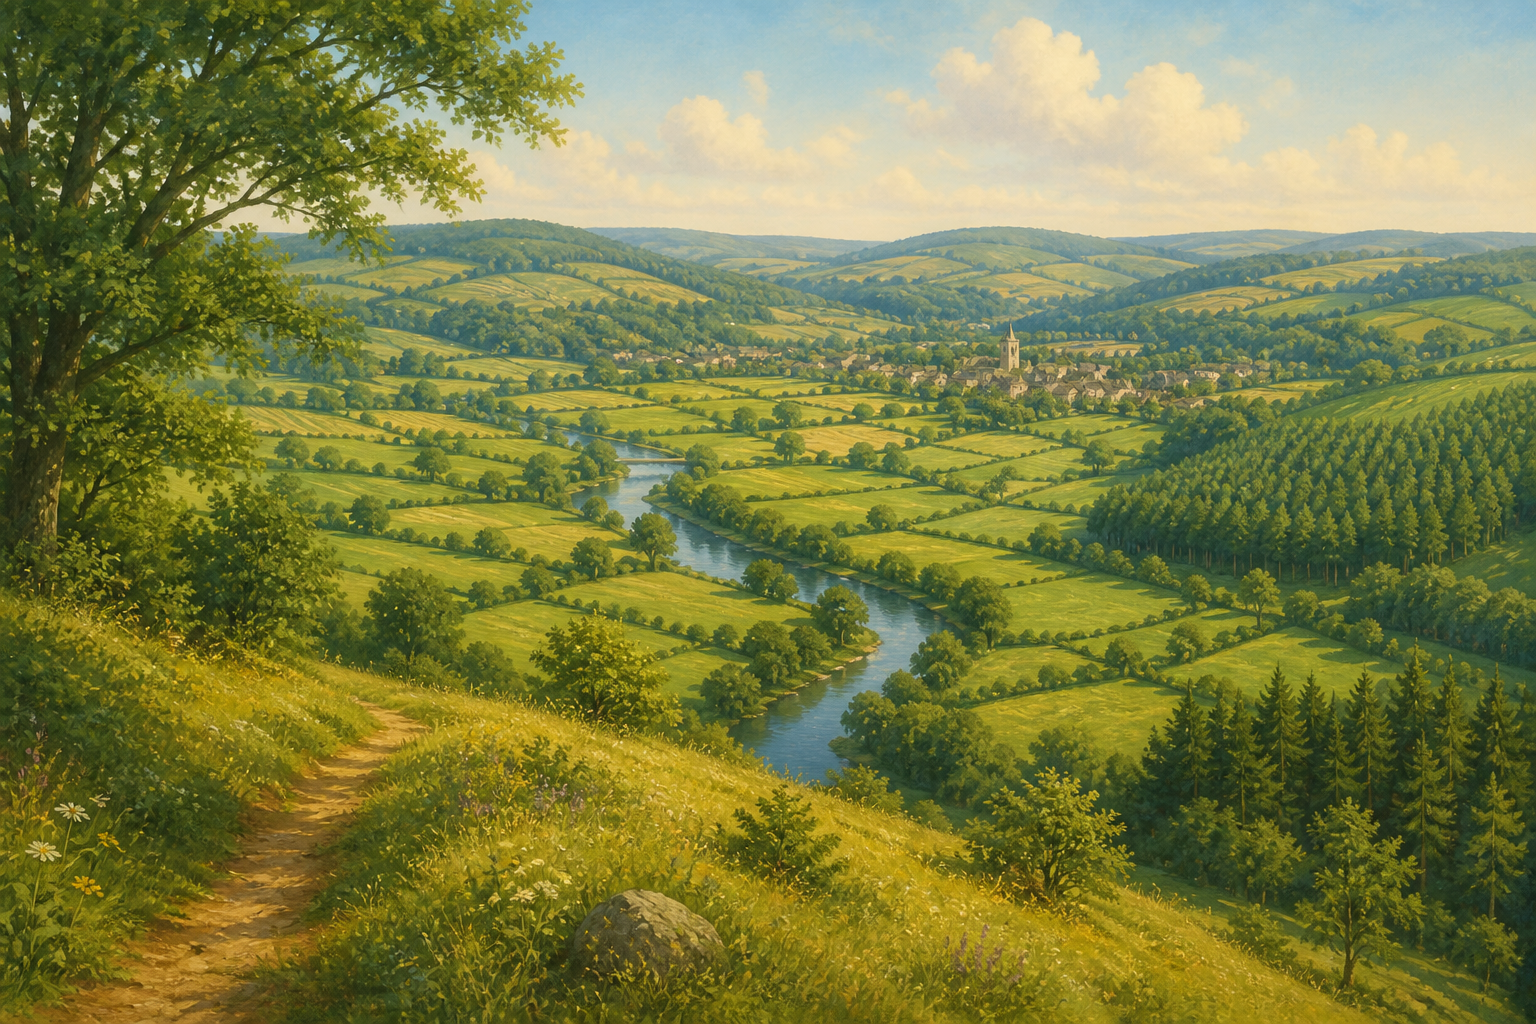
\includegraphics[width=0.62\linewidth]{images/book1/ai/g5-nature-valley.png}

{\small Pemandangan dari puncak bukit: ladang, pagar tanaman, \omterm{prop:g5:people-and-nature:managed}{hutan
kelolaan}, sungai yang diluruskan, desa --- sebuah bentang alam yang
bekerja, berumur berabad-abad.}
\end{omfigure}

\begin{remark}[Bukan penjahat, bukan pula patung taman]\label{rem:g5:people-and-nature:honest}
Akan keliru menceritakan kisah ini sebagai penghancuran belaka ---
pertanian memberi makan umat manusia, dan tanah pertanian yang berpagar
tanaman dapat kaya \omterm{def:g5:biodiversity:species}{spesies} (\cref{ex:g5:biodiversity:orchard}) --- dan
sama kelirunya berpura-pura bahwa pembentukan ulang itu tidak
berharga (\cref{prop:g5:biodiversity:loss} sudah mendaftarkan
tagihannya). Pertanyaan yang jujur tidak pernah ``menyentuh alam atau
tidak?'' melainkan ``bagaimana mengelola apa yang kita sentuh agar ia
terus bekerja --- bagi kita dan bagi seluruh jaringnya?''
\end{remark}

\section{Mengelola dengan baik dan mengelola dengan buruk}

\begin{example}[Dua cara bertani di sebuah lereng]\label{ex:g5:people-and-nature:twofarms}
Lereng A: satu ladang raksasa, pagar tanamannya dibongkar, tanahnya
telanjang sepanjang musim dingin. Hujan menghanyutkan tanah yang
longgar itu menuruni bukit; para penolong pada
\cref{ex:g5:biodiversity:orchard} tidak punya rumah; satu hama saja
dapat menyapu tanaman tunggalnya tanpa perlawanan. Lereng B: ladang
yang lebih kecil dengan pagar tanaman yang dipertahankan, tanah yang
tertutup sepanjang musim dingin, tanaman yang digilir tahun demi
tahun. Pagar tanamannya menahan tanahnya dan memondokkan para pemakan
hamanya; penggilirannya mengistirahatkan tanahnya. Kedua lereng itu
memberi makan manusia --- satu di antaranya masih akan melakukannya
seratus tahun lagi.
\end{example}

\begin{proposition}[Aturan pemakaian yang bertahan]\label{prop:g5:people-and-nature:lasting}
Pemakaian alam bertahan ketika ia menghormati tiga aturan:
\begin{enumerate}
  \item \emph{jangan mengambil lebih cepat daripada pembaruannya}:
        panenlah kayu pada laju pertumbuhan hutannya, tangkaplah \omterm{prop:g3:sorting-living-things:groups}{ikan}
        pada laju perkembangbiakan gerombolannya --- penangkapan \omterm{prop:g3:sorting-living-things:groups}{ikan}
        berlebihan pada \cref{prop:g5:biodiversity:loss} adalah
        pelanggaran aturan ini;
  \item \emph{pertahankan para pekerjanya}: kehidupan tanah,
        penyerbuk, pemakan hama --- jasa cuma-cuma pada
        \cref{exo:g5:biodiversity:11} --- membutuhkan rumahnya tetap
        dijaga;
  \item \emph{kembalikan apa yang kamu pinjam}: gelang kompos pada
        \cref{rem:g4:what-plants-need:soil}, pada setiap skala.
\end{enumerate}
\end{proposition}
\admitted

\begin{example}[Hitung-hitungan sang rimbawan]\label{ex:g5:people-and-nature:forester}
Hutan yang terkelola baik adalah bukti tertua bahwa aturan 1 berhasil:
rimbawan menghitung apa yang ditumbuhkan hutannya tiap tahun, lalu
menebang tidak lebih daripada itu. Hutannya lalu menghasilkan kayu
setiap tahun, selamanya --- sambil tetap menjadi hutan, dengan \omterm{prop:g3:sorting-living-things:groups}{burung}
hantu, rusa dan kumbangnya. Sebagian \omterm{prop:g5:people-and-nature:managed}{hutan kelolaan} di dunia sudah
dipanen dengan cara ini selama beratus-ratus tahun tanpa menyusut.
\end{example}

\section{Kota, dan memberi ruang lagi}

\begin{example}[Alam di dalam kota]\label{ex:g5:people-and-nature:city}
Sebuah kota tampak seperti lawan dari alam, namun ia juga sebuah
\omterm{def:g2:where-animals-live:habitat}{habitat} --- \omterm{def:g2:where-animals-live:habitat}{habitat} berbatu yang aneh. \omterm{prop:g3:sorting-living-things:groups}{Burung} walet bersarang di
``tebing'' beton, rubah berpatroli di tempat sampah, \omterm{def:g1:plants-around-us:plant}{tumbuhan} liar
membelah celah aspal. Dan penghuni kota dapat memperlebar
sambutannya: taman, atap hijau, \omterm{def:g3:flowers-fruits-seeds:parts}{bunga} balkon bagi lebah, kolam sekolah
pada \cref{ex:g2:where-animals-live:schoolpond}. Metode pada
\cref{met:g5:biodiversity:help} berhasil di antara gedung-gedung juga.
\end{example}

\begin{example}[Mengembalikan kelok sebuah sungai]\label{ex:g5:people-and-nature:river}
Sungai lembah yang diluruskan itu mengalir cepat dan membanjiri
daerah hilirnya dengan buruk; \omterm{prop:g3:sorting-living-things:groups}{ikan} dan capungnya pergi bersama
keloknya. Sekarang para insinyur kadang \emph{mengelokkan ulang}
sungai semacam itu: lengkung yang dipulihkan dan padang rumput basah
memperlambat airnya, menyimpan banjirnya, dan bangau pada
\cref{ex:g5:biodiversity:storks} menemukan padang rumputnya kembali.
Pengelolaan dapat berjalan mundur --- memperbaiki juga termasuk
mengelola.
\end{example}

\begin{method}[Menilai sebuah pemakaian alam]\label{met:g5:people-and-nature:judge}
Diberikan pemakaian tanah atau air apa pun --- sebuah pertanian, sebuah
perikanan, sebuah rencana jalan, sebuah kebun:
\begin{enumerate}
  \item tanyakan apa yang \emph{diambil}, dan apakah lebih cepat
        daripada pembaruannya (aturan 1);
  \item tanyakan \emph{rumah dan pekerja} apa yang dipertahankan atau
        hilang (aturan 2);
  \item tanyakan apa yang \emph{dikembalikan} --- dan buangan apa yang
        ditinggalkan (aturan 3);
  \item lalu nilailah: dapatkah hal ini berjalan seratus tahun lagi?
        Satu perubahan apa yang paling memperbaiki jawabannya?
\end{enumerate}
\end{method}

\section{Latihan}

\begin{exercise}[$\star$]\label{exo:g5:people-and-nature:1}
Sebutkan empat jenis bentang alam yang dibentuk manusia dari
\cref{prop:g5:people-and-nature:managed}, masing-masing dengan tujuan
pengelolaannya.
\end{exercise}

\begin{exercise}[$\star$]\label{exo:g5:people-and-nature:2}
Apa yang terjadi pada padang rumput yang berhenti dipangkas atau
digembalai?
\end{exercise}

\begin{exercise}[$\star$]\label{exo:g5:people-and-nature:3}
Nyatakan ketiga aturan pemakaian yang bertahan.
\end{exercise}

\begin{exercise}[$\star$]\label{exo:g5:people-and-nature:4}
Pada \cref{ex:g5:people-and-nature:twofarms}, daftarkan tiga perbedaan
antara kedua lerengnya, dan apa yang diubah tiap perbedaannya.
\end{exercise}

\begin{exercise}[$\star$]\label{exo:g5:people-and-nature:5}
Jelaskan hitung-hitungan sang rimbawan. Aturan yang mana itu, dan apa
yang dihasilkan hutannya sebagai balasan --- untuk berapa lama?
\end{exercise}

\begin{exercise}[$\star$]\label{exo:g5:people-and-nature:6}
Sebutkan tiga penghuni liar kota, dan ciri kota mana yang dipakai
masing-masing sebagai \omterm{def:g2:where-animals-live:habitat}{habitat}.
\end{exercise}

\begin{exercise}[$\star$]\label{exo:g5:people-and-nature:7}
Apa yang dipulihkan oleh pengelokan ulang sungainya --- bagi manusia,
dan bagi jaringnya?
\end{exercise}

\begin{exercise}[$\star$]\label{exo:g5:people-and-nature:8}
Cobalah: pilih satu pemandangan di dekat rumah --- jalan, ladang,
taman --- lalu daftarkan segala yang dikelola manusia di dalamnya,
seperti pada \cref{ex:g5:people-and-nature:valley}. Adakah yang
tertinggal tanpa dikelola?
\end{exercise}

\begin{exercise}[$\star\star$]\label{exo:g5:people-and-nature:9}
``Melindungi alam berarti tidak pernah menyentuhnya.'' Bahaslah dengan
memakai padang rumput yang dipangkas pada
\cref{prop:g5:people-and-nature:managed} --- sebuah \omterm{def:g2:where-animals-live:habitat}{habitat} yang
\emph{lenyap} tanpa sentuhan manusia --- dan
\cref{rem:g5:people-and-nature:honest}.
\end{exercise}

\begin{exercise}[$\star\star$]\label{exo:g5:people-and-nature:10}
Jalankan \cref{met:g5:people-and-nature:judge} atas lereng A pada
\cref{ex:g5:people-and-nature:twofarms}: aturan mana yang
dilanggarnya, dan satu perubahan apa yang paling memperbaikinya?
\end{exercise}

\begin{exercise}[$\star\star\star$]\label{exo:g5:people-and-nature:11}
Sebuah armada penangkap \omterm{prop:g3:sorting-living-things:groups}{ikan} melipatduakan tangkapannya selama lima
tahun yang gemilang; pada tahun keenam, gerombolan \omterm{prop:g3:sorting-living-things:groups}{ikannya} lenyap dan
armadanya menganggur. Jelaskan keenam tahun itu dengan aturan 1 ---
mengapa melanggarnya \emph{tampak} seperti keberhasilan pada mulanya?
Bandingkan dengan hitung-hitungan sang rimbawan yang berlawanan.
\end{exercise}
